\documentclass[11pt,aspectratio=169]{beamer}
\usetheme{CambridgeUS}
\beamertemplatenavigationsymbolsempty
\usepackage{fontspec}
\setsansfont{Junicode}
\usepackage{amsmath,mathtools}
\usepackage{hyperref}
\usepackage{graphicx}
\usepackage{xpatch}
\usepackage[export]{adjustbox}
\usepackage{pgfplots}
\usepackage{tikz}

\usetikzlibrary{shapes,calc,matrix,decorations.markings,decorations.pathreplacing,positioning, intersections,backgrounds,through,hobby,arrows.meta}
\usepackage{csquotes}
\usepackage[french]{babel}
\date[10/09/2024]{Nancy, 10 septembre 2024}
\author[Matthias \textsc{Gille Levenson}]{Journées d'Études \enquote{De la transcription manuelle participative des textes à la reconnaissance automatique de texte (ATR/HTR) : outils, théorie, pratiques.}\\~\\ Matthias \textsc{Gille Levenson}\\   {\scriptsize École nationale des chartes -- Centre Jean Mabillon \& École Normale Supérieure de Lyon -- CIHAM UMR 5648}\vspace{-.5cm}%\\ {\tiny prénom [point] gille [tiret] levenson [at] ens-lyon [point] org}\vspace{-.5cm}%
}
\title[De la donnée avant toute chose?]{De la donnée avant toute chose? Retour d'expérience de l'utilisation de l'HTR dans des projets d'édition et d'étude des textes médiévaux}
\titlegraphic{\vspace{-.5cm}\includegraphics[scale=0.18]{/home/mgl/Bureau/Travail/admin/logos/enc.png}\hspace{0.5cm}\includegraphics[scale=0.18]{/home/mgl/Bureau/Travail/admin/logos/ensl.png}\hspace{0.5cm}\includegraphics[scale=0.20]{/home/mgl/Bureau/Travail/admin/logos/logo-ciham.png}}


%\usepackage[labelformat=empty]{caption}
\setbeamertemplate{caption}{\insertcaption\par}

\usepackage[datamodel=thesis,citestyle=authoryear,isbn=true,
doi=true,backend=biber,language=french,url=true,sorting=nty,maxnames=99999, maxcitenames=3]{biblatex}
\renewbibmacro{in:}{}
\renewcommand*{\bibfont}{\tiny} 
% http://mcclinews.free.fr/latex/introbeamer/elements_contenu.html
%\xapptobibmacro{cite}{\setunit{\nametitledelim}\printfield{year}}{}{}
\addbibresource{biblio.bib}

\begin{filecontents*}{thesis.dbx}
\ProvidesFile{thesis.dbx}[2014/06/14 supervisor for theses]
\RequireBiber[3]
\DeclareDatamodelFields[type=list,datatype=name]{supervisor}
\DeclareDatamodelEntryfields[thesis]{supervisor}
\end{filecontents*}


\begin{filecontents*}{french-thesis.lbx}
\ProvidesFile{french-thesis.lbx}[2014/06/14 english for thesis]
\InheritBibliographyExtras{french}
\NewBibliographyString{supervision,jointsupervision}
\DeclareBibliographyStrings{%
inherit           = {french},
supervision       = {{dirigée par}{dir\adddotspace }},
jointsupervision  = {{codirigée par}{codir\adddotspace }},
}
\end{filecontents*}

\DeclareLanguageMapping{french}{french-thesis}

\newbibmacro*{thesissupervisor}{%
  \ifnameundef{supervisor}{}{%
    \ifnumgreater{\value{supervisor}}{1}
      {\bibstring{jointsupervision}}
      {\bibstring{supervision}}
    \printnames{supervisor}}}

\xpatchbibdriver{thesis}
  {\printfield{type}}
  {\printfield{type}
   \newunit
   \usebibmacro{thesissupervisor}}
  {\typeout{yep}}
  {\typeout{no}}
  
% https://tex.stackexchange.com/a/184878 ajout direction thèse

\let\cite\parencite



\AtBeginSection[]
{\begin{frame}
 \frametitle{}  
 \tableofcontents[currentsection,
                  hideothersubsections,
                  subsubsectionstyle=show/show/show/hide
                   ]
 \end{frame} 
 }



\setbeamertemplate{sections/subsections in toc}[square]
\setbeamertemplate{bibliography item}[sqare]
\setbeamertemplate{itemize item}[square]
\setbeamertemplate{enumerate item}[square]
\setbeamertemplate{itemize subitem}[square]





\renewcommand*{\dotFFN}{}
\newcommand{\astfootnote}[1]{%
\let\oldthefootnote=\thefootnote%
\setcounter{footnote}{0}%
\renewcommand{\thefootnote}{\fnsymbol{footnote}}%
\footnote{#1}%
\let\thefootnote=\oldthefootnote%
}








%\setbeameroption{show notes on second screen=right}
\setbeamerfont{note page}{size=\footnotesize}
\addtobeamertemplate{note page}{\setbeamerfont{itemize/enumerate subbody}{size=\tiny}}{}

\begin{document}
\maketitle





\begin{frame}
\frametitle{Plan} % Table of contents slide, comment this block out to remove it
\tableofcontents % Throughout your presentation, if you choose to use \section{} and \subsection{} commands, these will automatically be printed on this slide as an overview of your presentation
\end{frame}


\section{Introduction}
\begin{frame}{Expériences personnelles avec l'HTR}

\begin{itemize}
\item Pour de l'édition
\item Pour l'étude proprement dite du texte
\item Actuellement, pour des expériences de collation multilingue
\end{itemize}
\note{
\vfill
Idée de la communication
\begin{itemize}
\item Proposer un retour d'expérience
\item Donner des pistes et mes idées sur les bonnes pratiques en ATR dans une perspective plus globale d'étude et de traitement du texte patrimonial
\item De la donnée avant toute chose? Changement de paradigme avec l'apparition de l'apprentissage supervisé: il faut assumer ces changements et intégrer la nouvelle donne (ou la nouvelle donnée). Avant toute chose est donc à prendre au sens chronologique et non pas logique: la production du savoir et du texte reste prédominante.
\end{itemize}
\vfill}

\end{frame}

\begin{frame}{Édition critique}
\begin{figure}
\includegraphics[width=1\textwidth]{img/base_a.png}
\caption{Édition critique du \textit{Regimiento de los Prínçipes}, issue de collation automatisée. Les témoins A et Z sont issus d'HTR: \cite{gillelevenson_RegimientoPrincipesSa_2023} et \cite{gillelevenson_GeneralOpenDataset_2023}}
\end{figure}\note{
\vfill
Idée de la communication
\begin{itemize}
\item Travail sur une traduction castillane du \textit{De Regimine Principum} de Gilles de Rome.
\item Je parle depuis le point de vue d'un médiéviste, d'un philologue et d'un éditeur de textes patrimoniaux
\end{itemize}
\vfill}
\end{frame}


\begin{frame}{Études de la réception d'un manuscrit par ses marques de lecture}
\begin{figure}
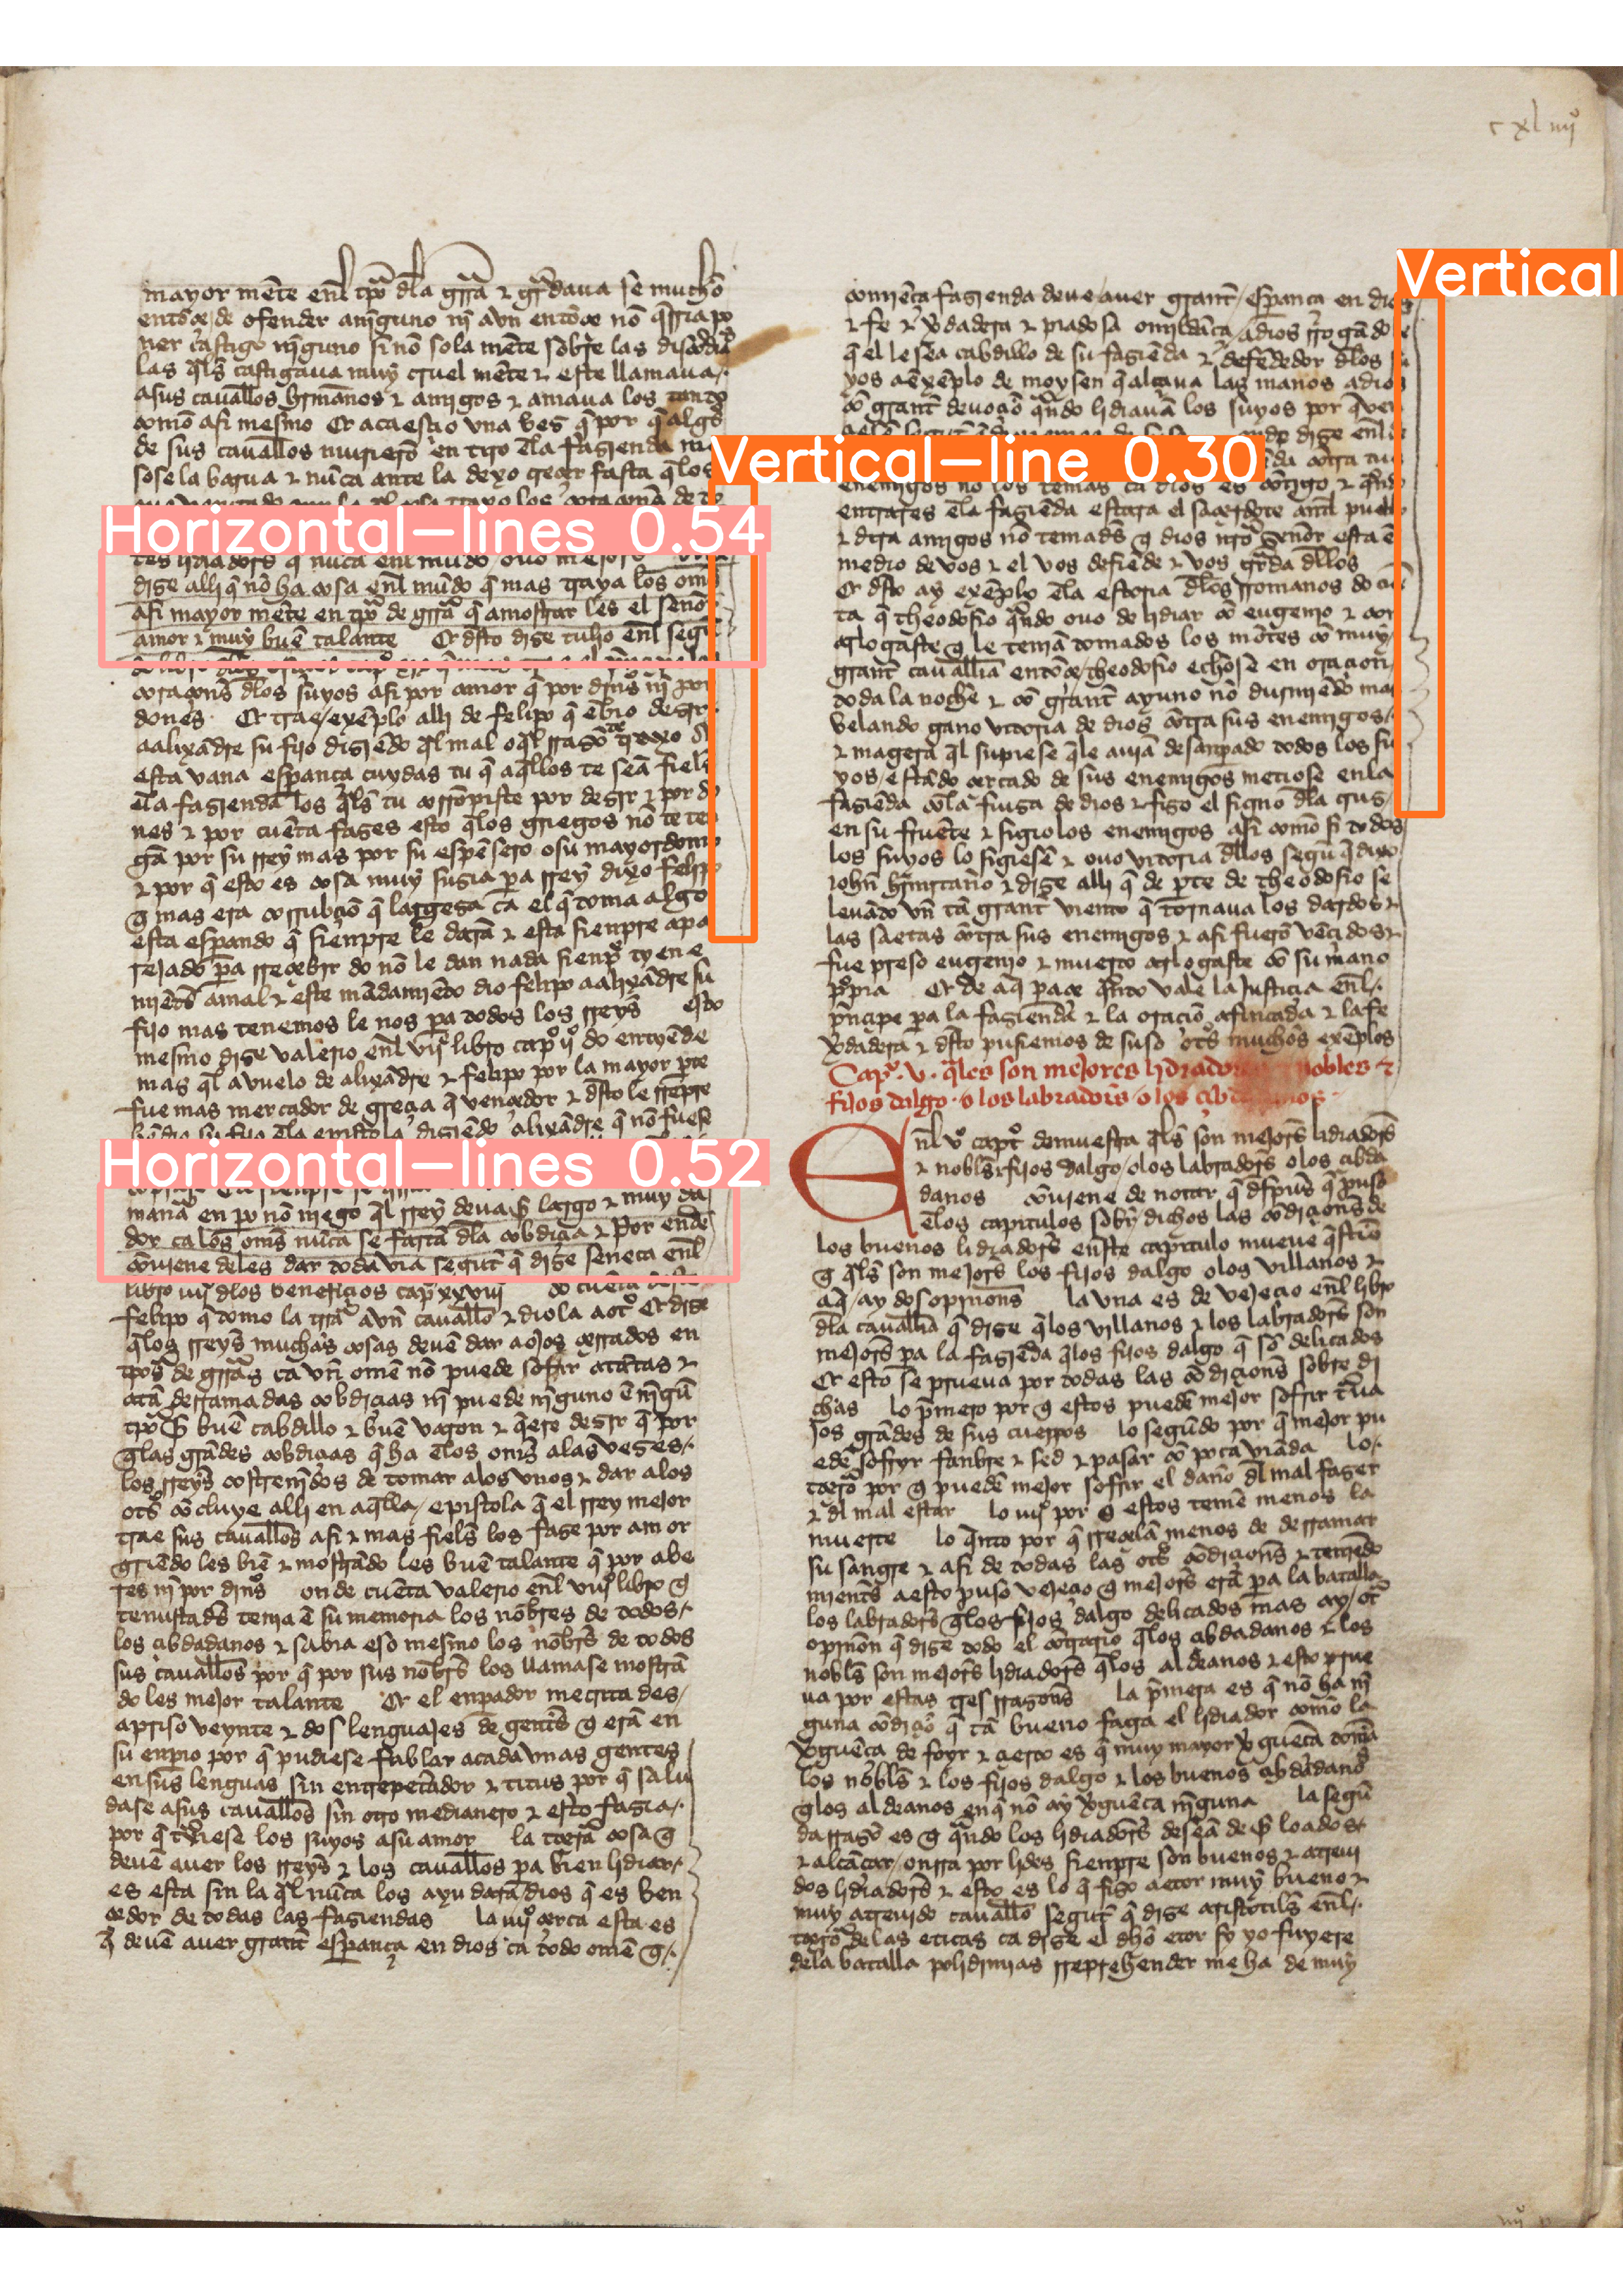
\includegraphics[width=.5\textwidth, trim={0 53cm 0 5cm}, clip]{img/YOLO_identification.png}
\caption{Identification automatisée  avec YOLO v5 \cite{redmon_YouOnlyLook_2016a} de zones de texte marquées par un lecteur. Escorial Ms. K.I.5, fol. 144r}
\end{figure}
\end{frame}


\begin{frame}{Rappels sur le fonctionnement (actuel) de l'HTR}

\begin{itemize}
\item Trois phases distinctes: segmentation en \textbf{zones}, segmentation en \textbf{lignes}, \textbf{transcription}
\pause\item Respecter les phases et bien découper le travail permet de gagner du temps \textit{in fine} et de produire des données de meilleure qualité
\pause\item Avec Kraken \cite{kiessling_KrakenUniversalText_2019}, pas de transcription globale du texte mais ligne par ligne
\end{itemize}
\end{frame}

\section{Phase de production des données}

\subsection{Penser la production en amont}

\begin{frame}{Penser la production en amont}
\begin{itemize}
\item Différencier et \textbf{hiérarchiser données et modèles} et privilégier les premières sur les seconds
\pause\item Se mettre d'accord en amont de la production sur des normes d'annotation:

	\begin{itemize}
	\pause\item Quelle typologie des zones et des lignes utiliser ? Identifier les titres de section ? Identifier toutes les zones ?
	\pause\item Comment transcrire ?
	\pause\item Que faire des abréviations ?
	\end{itemize}
	\pause\item Éviter à tout prix les modèles \enquote{boule de neige}:
\end{itemize}
\pause\begin{figure}
    \centering
    \includegraphics[width=.6\textwidth, trim={0 3.2cm 0 2cm},clip]{img/snowball.png}
    \caption{Un cas de modèle produit à partir de données hétérogènes, identifié par J.M. Fradejas \cite{pinche_CATMuSMedievalConsistentApproaches_2024}}
    \label{fig:coloseo}
\end{figure}
\note{
\vfill
\begin{itemize}
\item Question de pérennité: les données restent, les modèles disparaissent.
\end{itemize}
\vfill
}
\end{frame}


\subsection{CATMuS, un projet de production collaboratif de données d'ATR}

\begin{frame}
\begin{figure}
    \includegraphics[width=1\textwidth]{img/catmus_img.png}
\end{figure}
\begin{itemize}
\item Volonté autour de 2022 de réunir des producteur.ices de données (philologues) venant d'horizons distincts
\item Naissance du projet CATMuS pour \enquote{\textit{Consistent Approaches for Transcribing Manuscripts}}
\item Le corpus est récemment publié \cite{clerice_CATMuSMedievalMultilingual_2024a}
\end{itemize}\note{
\vfill
\begin{itemize}
\item Je parle ici au nom de l'équipe.
\end{itemize}
\vfill
}
\end{frame}


\begin{frame}{Statistiques sur le corpus CATMuS}
\begin{itemize}
\item Publié sur HuggingFace: \url{https://huggingface.co/datasets/CATMuS/medieval}
\item Recueil de 17 dépôts différents \textbf{homogénéisés} selon les normes du projet
\item Environ 175.000 lignes transcrites et intégralement corrigées (corpus \textit{gold})
\item 245 documents différents en 9 langues
\item Du \textsc{ix}\textsuperscript{e} au \textsc{xv}\textsuperscript{e} siècle, avec une prédominance du bas Moyen Âge (\textsc{xiii}\textsuperscript{e}-\textsc{xv}\textsuperscript{e} siècles)
\item Corpus encore biaisé en raison de l'histoire du projet
\pause\begin{figure}
    \includegraphics[width=.8\textwidth]{img/training_results.png}
\caption{Modèles produits à partir des données de CATMuS. \cite[16]{clerice_CATMuSMedievalMultilingual_2024a}}
\end{figure}
\end{itemize}\note{
\vfill
\begin{itemize}
\item Les biais: langue et genre littéraire; encore peu de sources pratiques et d'écritures cursives.
\item Résultats: c'est la théorie. On verra plus tard ce que ça donne en pratique
\end{itemize}
\vfill
}
\end{frame}


\begin{frame}{Une pomme de discorde: les abréviations}

\color{black}Notre point de vue est celui de philologues:
\begin{itemize}
\item Nous considérons la résolution des abréviations comme une tâche de TAL plutôt que de vision assistée par ordinateur \cite{clerice_CATMuSMedievalMultilingual_2024a}
\item La résolution via ATR pose des problèmes de \textbf{généralisation} et d'\textbf{adaptation}.
\end{itemize}
\note{
\vfill
\begin{itemize}
\item Généralisation: le développement des abréviations peut poser problème dans le cadre de corpus multilingue; les résultats sont moins bons en développant les abréviations
\item Adaptation: le développement des abréviations est dépendant du contexte linguistique et historique du document.
\end{itemize}
\vfill
}
\end{frame}


\begin{frame}{Le choix de la conservation des abréviations}
\color{black}Une norme de transcription \textbf{graphématique} \cite{stutzmann_PaleographieStatistiquePour_2010}:
\begin{center}
\begin{itemize}
\item Réduction des allographes au graphème
\item Réduction des allographes <i>/<j> et <u>/<v> à <i> et à <u>
\item Non développement des abréviations
\item Alignement sur les caractères proposés par la MUFI \cite{haugen_DealingGlyphsCharacters_2013}:\\ \url{https://mufi.info/}
\end{itemize}
\pause\begin{figure}
\includegraphics[width=.8\textwidth]{img/exemple_transcription.png}
\end{figure}
\end{center}
\end{frame}


\subsection{}


\begin{frame}{Concilier l'intérêt particulier et les besoins généraux}
\begin{center}
\begin{itemize}
\item Cette solution nous semble être le plus à même de \textbf{concilier besoins généraux et particuliers}
\item La question de l'\textbf{homogénéité des données} est fondamentale: manuel d'annotation et outils de contrôle (\url{https://github.com/PonteIneptique/choco-mufin} et \url{https://github.com/HTR-United/HTRVX})
\item La contrepartie est la nécessité de \textbf{travailler en aval} de l'acquisition du texte pour normaliser le texte
\item Le manuel en ligne est disponible: \url{https://catmus-guidelines.github.io/} (en cours de rédaction)
\end{itemize}
\end{center}
\note{
\vfill
\begin{itemize}
\item \textbf{Transition}: produire des données, c'est bien, mais comment faire après ? Le travail n'est pas du tout fini. Comment corriger le texte ? Comment gérer la segmentation ? Les abréviations ? Qu'est-ce qui change pour l'édition ? 
\end{itemize}
\vfill
}
\end{frame}

\section{Après l'HTR: tout change / rien ne change}

\subsection{Quand s'arrête la correction ?}
\begin{frame}{Quand s'arrête la correction ?}
\begin{center}
\begin{itemize}
\item La phase suivant la transcription automatisée sera généralement celle de la transformation en TEI
\item Plusieurs outils permettent de réaliser cette transformation: \url{https://github.com/Jean-Baptiste-Camps/ALTEI}, \url{https://github.com/chartes/alto2tei}, \url{https://github.com/matgille/alto_to_tei/}
\item Il restera des erreurs dans les données
\item Faut-il intégrer les corrections faites dans les données d'entraînement ? 
\item Si oui, cela suppose de penser en amont une modélisation en TEI qui soit \textbf{rétroconvertible}
\item En d'autres termes, il faudra conserver un premier état de TEI pseudo-diplomatique (conservation des \texttt{tei:lb})
\end{itemize}
\end{center}
\note{
\vfill
\begin{itemize}
\item \textbf{PASSER}
\item Suppose d'extraire les lignes pour pouvoir corriger ligne par ligne
\item La question étant la suivante: attend-on d'être sûr de la qualité de la transcription avant de transformer en TEI ? 
\end{itemize}
\vfill
}
\end{frame}


\begin{frame}{Assurer la rétroconvertibilité}
\begin{center}
\begin{figure}
\includegraphics[width=1\textwidth]{img/tei_retroconvertible.png}
\caption{Le document TEI avec des identifiants présents dans le fichier ALTO originel}
\end{figure}
\end{center}
\note{
\vfill
\begin{itemize}
\item \textbf{PASSER}
\end{itemize}
\vfill
}
\end{frame}


\begin{frame}{Assurer la rétroconvertibilité}
\begin{center}
\begin{figure}
\includegraphics[width=1\textwidth]{img/alto.png}
\caption{Le fichier ALTO d'origine}
\end{figure}
\end{center}
\note{
\vfill
\begin{itemize}
\item \textbf{PASSER}
\end{itemize}
\vfill
}
\end{frame}


\subsection{Structurer les documents}
\begin{frame}{Structurer les documents}
\begin{center}
\begin{itemize}
\item Classifier les zones et les lignes lors de la phase d'ATR peut permettre de faciliter la structuration (semi-)automatisée du document:
\begin{figure}
\includegraphics[width=.45\textwidth]{img/segmentation_lignes.png}
\caption{Classification des lignes suivant le vocabulaire contrôlé SegmOnto \cite{gabay_SegmOntoCommonVocabulary_2021}. En fuchsia: les lignes de type \texttt{DefaultLine}; en jaune, les lignes de type \texttt{Headingline:rubric}. Vat. Borg. 360, fol 190v.}
\end{figure}
\end{itemize}
\end{center}
\note{
\vfill
\begin{itemize}
\item La classification des zones de textes permet de ne s'intéresser qu'à des zones précises (la colonne, ou au contraire les titres courants par exemple).
\item On utilisera la première ligne de la rubrique (dans la zone de texte principal) pour identifier une borne de division (un chapitre par exemple), et ainsi de suite pour tout le document.
\item L'exemple donné ici est doublement problématique: le numéro de chapitre est erronné, ce qui peut poser problème si l'on utilise le texte pour numéroter les divisions; en second lieu, l'ordre des lignes est évident pour l'humain mais plus difficile à identifier pour la machine (mais on y arrive!), ce qui peut de même poser problème pour la structuration du texte.
\end{itemize}
\vfill
}
\end{frame}


\subsection{Identifier la césure à la ligne}
\begin{frame}{Identifier la césure à la ligne}
\begin{center}
\begin{itemize}
\item Dans les manuscrits médiévaux la césure à la ligne n'est pas systématiquement indiquée
\begin{figure}
\includegraphics[width=.32\textwidth]{img/Valladolid_251_17r.png}
\includegraphics[width=.32\textwidth]{img/CCC_MSS_283_14r.png}
\includegraphics[width=.27\textwidth]{img/Borgh_360_190r.png}
\includegraphics[width=.27\textwidth]{img/BNF_esp_36_1v.png}
\includegraphics[width=.27\textwidth]{img/BNE_958_14r.png}
\includegraphics[width=.27\textwidth]{img/Valencia_BH-Ms-0594_23r.png}
\caption{Valladolid, 251 fol. 17r; Cambridge, Corpus Christi College, MS 283, fol 14r; Vatican, Borg. 360, fol. 190r;  BNF Esp 36, fol 1v;  BNE MSS/958, fol. 14r; Valencia BH Ms 0594, fol. 23r}
\end{figure}
\end{itemize}
\end{center}
\note{
\vfill
\begin{itemize}
\item On montre des cas d'indications, des cas de non-indication (un texte en castillan, trois en latin; deux manuscrits ibériques, un manuscrit anglais, et un manuscrit italien).
\item Dans le corpus manuscrit castillan du 15e siècle, c'est assez peu commun, alors que l'indication sera plus fréquente en latin par exemple. 
\item La tâche d'identification de la césure me semble raisonnablement automatisable
\item Cette tâche ne peut être actuellement efficacement traitée par les outils d'ATR comme Kraken, étant donné que l'outil ne fonctionne que ligne par ligne sans contexte.
\end{itemize}
 
\vfill
}
\end{frame}

\begin{frame}{Identifier la césure}
\color{black}
\begin{figure}[htp!]
\begin{center}
\includegraphics[width=0.5\textwidth]{img/ligne_1.png}
\includegraphics[width=0.5\textwidth]{img/ligne_2.png}
\includegraphics[width=0.5\textwidth]{img/ligne_3.png}
%\caption{Ms. 251, Valladolid, Bib. Santa Cruz, fol. 3v}
\end{center}
\end{figure}
\begin{center}
\pause adios ⁊ ganarã gloĩa ꝑdurable ¶ Et pu\\
es q̃ asy es los bieñs deꝑtẽ se en una ma\\
n̾a Ca alguõs dellos son muy peq̃nos\\
{\color{black}$\Updownarrow$}\\
 adios ⁊ ganarã gloĩa ꝑdurable ¶ Et \underline{pues} es q̃ asy es los bieñs deꝑtẽ se en una \underline{man̾a} Ca alguõs dellos son muy peq̃nos
\end{center}
\pause Voir \cite{clerice_EvaluatingDeepLearning_2020} et \url{https://github.com/matgille/boudams_like_tokenizer}
\note{
\vfill
Il suffit donc d'associer deux à deux les lignes (faire des bigrames de lignes) afin d'identifier si la chaîne de caractère de fin de ligne correspond aussi à une fin de mot.
\vfill
}
\end{frame}

\subsection{Résoudre les abréviations}
\begin{frame}{Résoudre les abréviations}
\begin{center}
\begin{itemize}
\item Le plus \enquote{simple} est d'utiliser une table de conversion à base de règles
\item Suppose de connaître en amont toutes les abréviations et cas possibles \textbf{en contexte}
\item Un peu laborieux quand le volume de documents différents est important
\end{itemize}
\begin{figure}
\includegraphics[width=0.5\textwidth]{img/table_abreviation.png}
\caption{Table d'abréviation. \texttt{<SOT>} et \texttt{<EOT>} viennent marquer un début et/ou une fin de mot}
\end{figure}
\end{center}
\note{
\vfill
\begin{itemize}
\item Un travail en cours à préciser; encore des irrégularités dans la table
\item les choix
\end{itemize}
\vfill
}
\end{frame}


\subsection{Et l'édition critique ?}

\begin{frame}{Et l'édition critique ?}
\color{black}\only<1>{L'ATR appelle assez naturellement des méthodes de collation automatisée du texte}
\only<2>{\begin{center}
\begin{figure}
\includegraphics[width=.85\textwidth]{img/avant_correction.png}
\caption{Table d'alignement avant la phase de correction, après segmentation et résolution des abréviations. Gilles de Rome, \textit{De Regimine Principum}, chapitre 1.2.2}
\end{figure}
\end{center}}
\note{
\vfill
\begin{itemize}
\item Un projet en cours d'édition multilingue qui commence avec la collation du texte latin, sur un quinzaine ou une vingtaine de témoins manuscrits et imprimés
\item 
Un texte difficilement exploitable, en sortie d'HTR désabrévié, sans correction et avec affinage minimal des modèles. Il reste du travail sur les modèles !
\end{itemize}
\vfill
}
\end{frame}

\begin{frame}{Et l'édition critique ?}
\begin{center}
\begin{figure}
\includegraphics[width=1\textwidth]{img/apres_correction.png}
\caption{Table d'alignement après la phase de correction. Gilles de Rome, \textit{De Regimine Principum}, chapitre 1.2.1}
\end{figure}
\end{center}\note{
\vfill
\begin{itemize}
\item On a vu la théorie, voici la pratique
\item Il reste encore des erreurs mais le texte est exploitable; le but n'est ici pas éditorial mais stemmatologique 
\item Un mot sur la typologie des variantes: elle s'appuie sur les annotation lexicales (lemmes): il suffit d'une erreur de lemmatisation (dûe à une variante graphique) pour fausser la classification et créer du faux positif, d'où une tâche dont la difficulté augmente avec le nombre de témoins.
\end{itemize}
\vfill
}
\end{frame}


\section{Conclusions}

\begin{frame}
\begin{itemize}
\item Penser en amont les principes d'annotation est fondamental
\begin{itemize}
\item Identifier les intérêts et les inconvénients de chaque choix en terme de balance intérêt particulier / intérêt général
\item Lancer de courtes campagnes test pour mettre à l'épreuve les choix d'annotation
\item Identifier le type d'information nécessaire aux étapes ultérieures de traitement du texte manuscrit ou imprimé: penser l'ensemble de la production des données et pas seulement l'HTR pour l'HTR
\item Se mettre en conformité (ou pas) avec les normes existantes et le documenter clairement
\end{itemize}
\item Du travail reste à mener
\begin{itemize}
\item Sur tout la chaîne post-ATR afin d'arriver à un texte final plus propre
\item Et plus particulièrement pour la collation
\item Quid de l'accumulation du bruit avec la multiplication des étapes?
\end{itemize}
\end{itemize}\note{
\vfill
\begin{itemize}
\item S'appuyer sur un Plan de Gestion de Données (PGD) ?
\end{itemize}
\vfill
}
\end{frame}


\begin{frame}{Merci !}
\begin{center}
\color{black}Merci de votre attention !
\begin{itemize}
\item Diapos: \url{https://github.com/matgille/Comm_Nancy_sept_2024}
\end{itemize}
\end{center}
\end{frame}



\begin{frame}[allowframebreaks]{Références}
\printbibliography
\end{frame}

\end{document}
